\documentclass{beamer}
\usepackage[utf8]{inputenc}

\usepackage{fourier} %font utopia imported
\usetheme{Madrid}
\usecolortheme{default}

%------------------------------------------------------------
%This block of code defines the information to appear in the
%Title page
\title[Synthesizing Co-Simulation Algorithms] %optional
{Synthesizing and Verifying Orchestration Algorithms}
\date{\today}
\usepackage{booktabs}
\usepackage{natbib}
\usepackage{multicol}
\usepackage{listings}
\usepackage{environ}
\usepackage{graphicx}
\usepackage{amsfonts}
\usepackage{amsmath}
\usepackage{amssymb}
\usepackage{stmaryrd}
\usepackage{amstext}
\usepackage{semantic}
\usepackage{semantic}
\usepackage{algorithm}
\usepackage{algpseudocode}
\usepackage{etoolbox}
\usepackage{paralist}
\usepackage{verbatim}


\usepackage[capitalise,nameinlink]{cleveref}

% Comments

\newcommand{\simon}[1]{%
  {\scriptsize
      \textbf{\textcolor{red}{Simon: #1}}
  }%
}%

\newcommand{\peter}[1]{%
  {\scriptsize
      \textbf{\textcolor{blue}{Peter: #1}}
  }%
}%

% Paper specific notation

\setlength{\intextsep}{10pt}

\crefname{problem}{problem}{problems}

\newcommand{\inputV}{v}
\newcommand{\consistent}{\ensuremath{\mathit{Consistent}}}
\newcommand{\remaining}{\ensuremath{\mathit{Remaining}}}
\newcommand{\dontcare}{\_}
\newcommand{\defined}{\ensuremath{\mathit{defined}}}
\newcommand{\undefined}{\ensuremath{\mathit{undefined}}}
\newcommand{\properties}{P}
\newcommand{\satisfies}{\vDash}
\newcommand{\simulator}{\mathcal{A}}
\newcommand{\Induced}[2]{\llbracket #1 \rrbracket_{#2}}
\newcommand{\timebase}{\setreal_{\geq 0}}
\newcommand{\stepbase}{\setreal_{> 0}}
\newcommand{\variables}[1]{\mathit{VAR_{#1}}}
\newcommand{\stateset}[1]{S_{#1}}
\newcommand{\runstate}[1]{S^{R}_{#1}}
\newcommand{\state}[1]{s_{#1}}
\newcommand{\inputs}[1]{U_{#1}}
\newcommand{\parameters}[1]{P_{#1}}
\newcommand{\inputvar}[1]{u_{#1}}
\newcommand{\outputs}[1]{Y_{#1}}
\newcommand{\outputvar}[1]{y_{#1}}
\newcommand{\mayReject}{M}
\newcommand{\backtrack}{B}
\newcommand{\values}{\mathcal{V}}
\newcommand{\valuesExchanged}{\mathcal{V_{E}}}
\newcommand{\true}{\mathit{true}}
\newcommand{\false}{\mathit{false}}
\newcommand{\feedthrough}[1]{F_{#1}}
\newcommand{\reactivity}[1]{R_{#1}}
\newcommand{\fset}[1]{\mathtt{set}_{#1}}
\newcommand{\fget}[1]{\mathtt{get}_{#1}}
\newcommand{\fdoStep}[1]{\mathtt{step}_{#1}}
\newcommand{\fpreset}[1]{\mathtt{preSet}_{#1}}
\newcommand{\fpreget}[1]{\mathtt{preGet}_{#1}}
\newcommand{\fpredoStep}[1]{\mathtt{preStep}_{#1}}
\newcommand{\ftime}{\mathtt{ftime}}
\newcommand{\maxStep}[1]{\mathtt{h}_{#1}}
\newcommand{\timestamp}[1]{\varphi(#1)}
\newcommand{\feedsto}[2]{U_{#1}^{#2}}
\newcommand{\CheckCon}{\mathit{CheckConv}}
\newcommand{\stepfound}{\mathit{Step\_found}}
\newcommand{\valuations}{\mathit{V}}
\newcommand{\valuation}{\mathit{v}}


\newcommand{\dom}[1]{\mathit{dom(#1)}}
\newcommand{\algebraic}[1]{\mathit{algebraic_{#1}}}

 

\newcommand{\precondition}{\mathit{Pre}}


\newcommand{\complexity}{Com}
\newcommand{\master}{\mathcal{A}}
\newcommand{\alloutputs}{Y}
\newcommand{\allfeedthroughs}{F}
\newcommand{\allreactivity}{R}
\newcommand{\alldelayed}{D}

\newcommand{\allcontracts}{\mathcal{C}}
\newcommand{\coupling}{L}
\newcommand{\allinputs}{U}
\newcommand{\fmus}{C}
\newcommand{\fmusLoop}{C_{loop}}
\newcommand{\sequence}[1]{\pargroup{#1}}
\newcommand{\functioncall}{f}
\newcommand{\initcall}{I}
\newcommand{\allfunctioncalls}{F}
\newcommand{\fmu}[1]{\texttt{#1}}
\newcommand{\signal}[1]{\texttt{#1}}
\newcommand{\before}[2]{\ensuremath{#1 \twoheadrightarrow #2}}
\newcommand{\ibefore}[2]{\ensuremath{#1 \rightarrow #2}}
\newcommand{\after}[1]{{#1}'}
\newcommand{\aftern}[2]{{#1}^{(#2)}}
\newcommand{\stateafter}[2]{\ensuremath{\state{#1}^{(#2)}}}
\newcommand{\minstep}{\ensuremath{h_{min}}}


\newcommand{\etime}{\ensuremath{E}}

\newcommand{\verifier}{\mathit{Verifier}}

\newcommand{\turnOn}{\mathit{TurnPreconditionsOn()}}
\newcommand{\turnOff}{\mathit{TurnPreconditionsOff()}}

\newtheorem{procedure}{Procedure}{}
\newtheorem{assumption}{Assumption}{}

\newtheorem{experiment}{Experiment}{}

\algrenewcommand\alglinenumber[1]{\scriptsize #1:}% Adapt size of line numbers in algorithm

\algnewcommand\algorithmicforeach{\textbf{for each}}
\algdef{S}[FOR]{ForEach}[1]{\algorithmicforeach\ #1\ \algorithmicdo}
% New definitions
\algnewcommand\algorithmicswitch{\textbf{switch}}
\algnewcommand\algorithmiccase{\textbf{case}}
\algnewcommand\algorithmicassert{\texttt{assert}}
\algnewcommand\Assert[1]{\State \algorithmicassert(#1)}%
% New "environments"
\algdef{SE}[SWITCH]{Switch}{EndSwitch}[1]{\algorithmicswitch\ #1\ \algorithmicdo}{\algorithmicend\ \algorithmicswitch}%
\algdef{SE}[CASE]{Case}{EndCase}[1]{\algorithmiccase\ #1}{\algorithmicend\ \algorithmiccase}%
\algtext*{EndSwitch}%
\algtext*{EndCase}%



% Generic stuff

\newcommand{\footurl}[1]{\footnote{\url{#1}}}

% Math
\newcommand{\brackets}[1]{\ensuremath{ \left[ #1 \right] }}
\newcommand{\tuple}[1]{\ensuremath{ \left\langle #1 \right\rangle }}
\newcommand{\set}[1]{\ensuremath{ \left\{ #1 \right\}}}
\newcommand{\system}[1]{\ensuremath{ \begin{cases} #1 \end{cases}}}
\newcommand{\rightgroup}[1]{\ensuremath{ \left. \begin{matrix} #1 \end{matrix} \right\} } }
\newcommand{\pargroup}[1]{\ensuremath{ \left( #1 \right)}}
\newcommand{\inv}[1]{\ensuremath{\pargroup{ #1 }^{-1}}}
\newcommand{\dert}[1]{\ensuremath{ \dot{#1} }}
\newcommand{\ddert}[1]{\ensuremath{ \ddot{#1} }}
\newcommand{\partialder}[2]{\ensuremath{ \frac{\partial#1}{\partial#2} }}
\newcommand{\setreal}[0]{\ensuremath{\mathbb{R}}}
%\newcommand{\setbool}[0]{\ensuremath{\mathit{Bool}}}
\newcommand{\setnat}[0]{\ensuremath{\mathbb{N}}}
\newcommand{\norm}[1]{\left\lVert#1\right\rVert}
\newcommand{\bnorm}[1]{\big\lVert#1\big\rVert}
\newcommand{\abs}[1]{\left|#1\right\|}
\newcommand{\xs}[2]{\ensuremath{#1^{\left[#2\right]}}}
\newcommand{\infinitynorm}[1]{\left\lVert#1\right\rVert_\infty}


\newcommand{\vectorOne}[1]{\brackets{%
\begin{matrix}
  #1
 \end{matrix}%
}}
\newcommand{\vectorTwo}[2]{\brackets{%
\begin{matrix}
  #1 \\
  #2
 \end{matrix}%
}}
\newcommand{\vectorThree}[3]{\brackets{%
\begin{matrix}
  #1 \\
  #2 \\
  #3
 \end{matrix}%
}}
\newcommand{\vectorFour}[4]{\brackets{%
\begin{matrix}
  #1 \\
  #2 \\
  #3 \\
  #4
 \end{matrix}%
}}
\newcommand{\vectorFive}[5]{\brackets{%
\begin{matrix}
  #1 \\
  #2 \\
  #3 \\
  #4 \\
  #5
 \end{matrix}%
}}
\newcommand{\vectorSix}[6]{\brackets{%
\begin{matrix}
  #1 \\
  #2 \\
  #3 \\
  #4 \\
  #5 \\
  #6
 \end{matrix}%
}}
\newcommand{\vectorSeven}[7]{\brackets{%
\begin{matrix}
  #1 \\
  #2 \\
  #3 \\
  #4 \\
  #5 \\
  #6 \\
  #7
 \end{matrix}%
}}
\newcommand{\vectorEight}[8]{\brackets{%
\begin{matrix}
  #1 \\
  #2 \\
  #3 \\
  #4 \\
  #5 \\
  #6 \\
  #7 \\
  #8
 \end{matrix}%
}}

\newenvironment{aligneq*}%
{
\begin{equation*}
\begin{aligned}
}{
\end{aligned}
\end{equation*}
}

\newenvironment{aligneq}%
{
\begin{equation}
\begin{aligned}
}{
\end{aligned}
\end{equation}
}



%enable \cref{...} and \Cref{...} instead of \ref: Type of reference included in the link
%Nice formats for \cref
\usepackage{iflang}
\IfLanguageName{ngerman}{
  \crefname{table}{Tab.}{Tab.}
  \Crefname{table}{Tabelle}{Tabellen}
  \crefname{figure}{\figurename}{\figurename}
  \Crefname{figure}{Abbildungen}{Abbildungen}
  \crefname{equation}{Gleichung}{Gleichungen}
  \Crefname{equation}{Gleichung}{Gleichungen}
  \crefname{listing}{\lstlistingname}{\lstlistingname}
  \Crefname{listing}{Listing}{Listings}
  \crefname{section}{Abschnitt}{Abschnitte}
  \Crefname{section}{Abschnitt}{Abschnitte}
  \crefname{paragraph}{Abschnitt}{Abschnitte}
  \Crefname{paragraph}{Abschnitt}{Abschnitte}
  \crefname{subparagraph}{Abschnitt}{Abschnitte}
  \Crefname{subparagraph}{Abschnitt}{Abschnitte}
}{
  \crefname{section}{Sect.}{Sect.}
  \Crefname{section}{Section}{Sections}
  \crefname{listing}{\lstlistingname}{\lstlistingname}
  \Crefname{listing}{Listing}{Listings}
}
\crefname{section}{Sect.}{Sect.}
\Crefname{section}{Section}{Sections}
\crefname{listing}{\lstlistingname}{\lstlistingname}
\Crefname{listing}{Listing}{Listings}

\crefname{assumption}{Assumption}{Assumptions}


% update later with official instructions from Springer
\def\orcidID#1{${}^{\smash{\href{https://orcid.org/#1}{\protect\raisebox{-1.25pt}{\protect
\includegraphics{images/orcid_color-eps-converted-to}}}}}$}




\urlstyle{same}
\author[Thrane, S.] % (optional)
{Simon Thrane Hansen \\ Ph.D. Student AU}


\date[AU 2021] % (optional)
{\today}

%\logo{\includegraphics[height=1.5cm]{lion-logo.jpg}}

%End of title page configuration block
%------------------------------------------------------------



%------------------------------------------------------------
%The next block of commands puts the table of contents at the 
%beginning of each section and highlights the current section:


%------------------------------------------------------------
\begin{document}

%The next statement creates the title page.
\frame{\titlepage}

\begin{frame}{Overview}
    \tableofcontents
\end{frame}

\section{Co-simulation}
\begin{frame}{Co-Simulation 101}
    \begin{itemize}
        \item Model-based development approach.
        \item A Simulation technique to explore the behavior of a CPS.
        \item Different subsystem/models are modeled and developed in specialized tools (different domains).
        \item The subsystems are connected and simulated for the global system behavior.
    \end{itemize}
    \begin{figure}    
        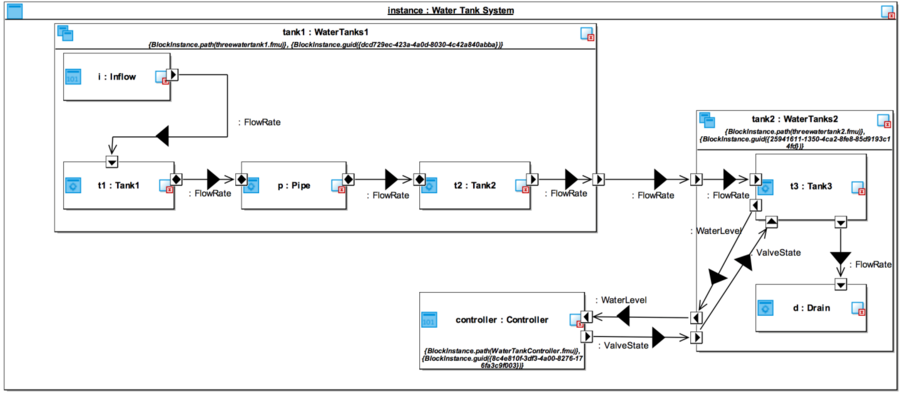
\includegraphics[width=0.6\textwidth]{images/co-simulation.png}
    \end{figure}
\end{frame}

\begin{frame}{Running a co-simulation}
    \begin{itemize}
        \item The simulation units (SU) are coupled together.
        \item Exchanging values between the SUs and calculating new states (behavioral trace) of each SU.
        \item An orchestrator drives the simulation.
        \item The combined behavioral trace is the co-simulation.
        \item The co-simulation \textbf{should} represent the real system.
    \end{itemize}
    \begin{figure}    
        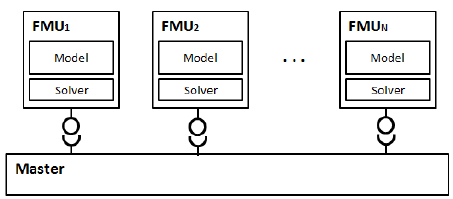
\includegraphics[width=0.55\textwidth]{images/master.png}
    \end{figure}
\end{frame}

\begin{frame}{The orchestrator is an algorithm!}
    \begin{itemize}
        \item Describes how the SU should act during the simulation.
        \item How and when are data exchanged - the communication points
        \item When are future states calculated
        \item The co-simulation result can be extremely affected by the algorithm!
    \end{itemize}

    \begin{columns}[T] % align columns
        \begin{column}{.48\textwidth}
            \begin{algorithm}[H]
                \caption{Step function}
                \label{alg:algorithm_simpleexample}
                \begin{algorithmic}[1]
                  \scriptsize
                  \State $\stateafter{b}{s+H} \gets \fdoStep{b}(\stateafter{b}{s}, H)$
                  \State $g_v \gets \fget{b}(\stateafter{b}{s+H}, \outputvar{b})$
                  \State $\stateafter{a}{s} \gets \fset{a}(\stateafter{a}{s}, \inputvar{g}, g_v)$
                  \State $\stateafter{a}{s+H} \gets \fdoStep{a}(\stateafter{a}{s}, H)$
                  \State $f_v \gets \fget{a}(\stateafter{a}{s+H}, \outputvar{f})$
                  \State $\stateafter{b}{s+H} \gets \fset{b}(\stateafter{b}{s+H}, \inputvar{f}, f_v)$
                \end{algorithmic}
              \end{algorithm}
    \end{column}%
    \hfill%
    \begin{column}{.48\textwidth}
        \begin{figure}    
            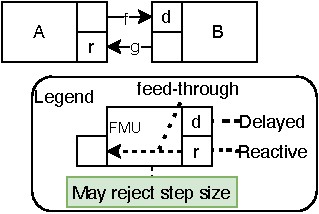
\includegraphics[width=0.9\textwidth]{images/simple_example_legend.pdf}
        \end{figure}
    \end{column}%
    \end{columns}
\end{frame}

\begin{frame}{What can make a co-simulation incorrect?}
    \begin{itemize}
        \item An error in an SU
        \begin{itemize}
            \item Implementation
            \item Conceptual
        \end{itemize}
        \item An incorrect orchestration algorithm
        \begin{itemize}
            \item Values are not exchanged optimally.
            \item Algebraic loops (Cycle dependencies) are not solved.
            \item The SUs do not move in lockstep.
        \end{itemize}
    \end{itemize}
    \textbf{My focus} is on detecting incorrect algorithms and creating correct ones!
\end{frame}

\begin{frame}{Co-simulation algorithms, why bother?}
    Co-simulation is a technique with huge potential - supported by more than 50 tools \footnote{\url{https://fmi-standard.org/tools/}}!
    \begin{itemize}
        \item Nobody can use an incorrect simulation result.
        \item A simulation can run for weeks - trial and error might take ages\dots
        \item Some errors can be hard to debug for domain experts. 
        \item The algorithm should be tailored to the specific scenario for efficiency and verification purposes.
    \end{itemize}

    \begin{figure}[htb]
        \centering
          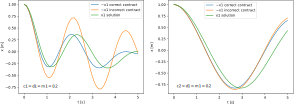
\includegraphics[width=0.9\textwidth]{images/merged_results_inkscape}
          \caption{Example results.}
          \label{fig:merged_results_inkscape}
      \end{figure}
\end{frame}

\begin{frame}{How do we do create such algorithms?}
    We need a formal definition of a co-simulation scenario and a correct co-simulation algorithm.
    \begin{enumerate}
        \item Co-simulation:
        \begin{itemize}
            \item SUs and their characteristics
            \item The couplings
        \end{itemize}
        \item Co-simulation algorithm
        \begin{itemize}
            \item How are values exchanged.
            \item When are new states calculated. 
            \item How are algebraic loops solved.
            \item The SUs should move in lockstep.
            \item Consist of an Initialization procedure and a \underline{co-sim step procedure}.
        \end{itemize}
    \end{enumerate}
\end{frame}

\begin{frame}{Co-Simulation Scenario}
    \begin{figure}    
        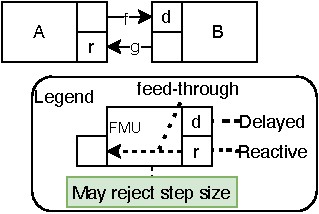
\includegraphics[width=0.4\textwidth]{images/simple_example_legend.pdf}
    \end{figure}
    \begin{itemize}
        \item Feed-through - a contract between input and output at all times.
        \item Couplings - a contract between output and input at all times.
        \item The SUs
        \item Which SUs may refuse to calculate a future state.
        \item Input approximation functions
    \end{itemize}
\end{frame}

\begin{frame}{Description of a Scenario}
    We describe scenarios like this:
    \begin{figure}
        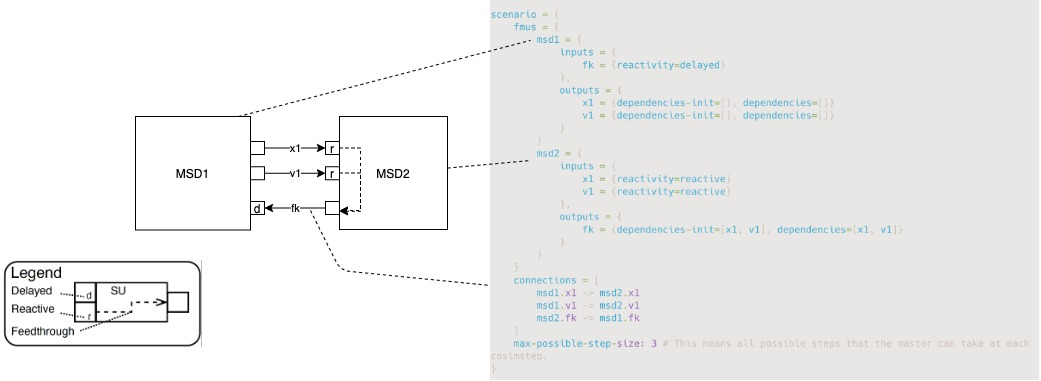
\includegraphics[width=1\textwidth]{images/scenario-generation.jpg}
    \end{figure}
\end{frame}

\begin{frame}{Simulation Unit}
    \begin{itemize}
        \item A dynamical system - a state that evolves.
        \item Interact with the environment through couplings on input and outputs.
        \item Can calculate its future state within in the interval: $[t,t+h]$. 
        \item Adheres to a well-defined interface that hides away the IP.
        \item A future state is calculated using assumptions on the input values between communication points - the most significant source of error in the simulation! 
    \end{itemize}

    \begin{columns}[T] % align columns
        \begin{column}{.48\textwidth}
            Extrapolation (Delayed inputs):
            \begin{figure}    
                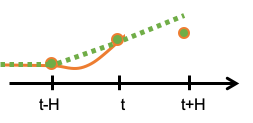
\includegraphics[scale=0.6]{images/extrapolation.png}
            \end{figure}
    \end{column}%
    \hfill%
    \begin{column}{.48\textwidth}
        Interpolation (Reactive inputs):
        \begin{figure}    
            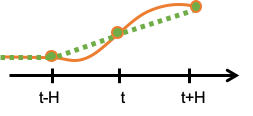
\includegraphics[scale=0.6]{images/interpolation.png}
        \end{figure}
    \end{column}%
    \end{columns}
\end{frame}

\begin{frame}
    \frametitle{The SU interface}
    \begin{itemize}
        \item Inputs with contract information (R/D).
        \item Outputs with internal dependencies.
        \item Current Time
        \item Actions:
        \begin{itemize}
            \item \textit{Get} for obtaining a value on an output.
            \item \textit{Set} for setting a value on an input.
            \item \textit{Step} for calculating a future state.
            \item \textit{Save} for saving the current state.
            \item \textit{Restore} for setting the current state to a previous one.
        \end{itemize}
    \end{itemize}
\end{frame}

\begin{frame}{Criteria for a correct algorithm}
    \begin{itemize}
        \item Termination and time-progression.
        \item The communication points should minimize the error of the input approximation.
        \item The SUs should move in lockstep, and step rejection should be corrected.
        \item Algebraic loops should be stabilized - obtaining a fixed-point.
    \end{itemize}

    \begin{figure}    
        \centering
        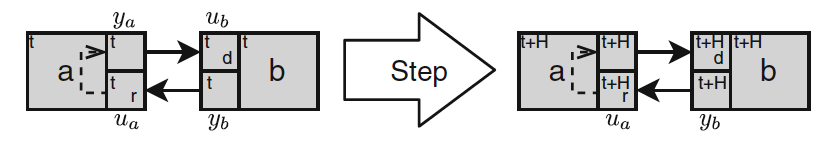
\includegraphics[width=0.9\textwidth]{images/cosimulation_algortihm.png}
        \caption{Gomes et al. 2020 - Generation of Co-simulation Algorithms Subject to Simulator Contracts}
    \end{figure}
\end{frame}

\section{Synthesizing an orchestration algorithm}
\begin{frame}{Synthesizing a orchestration algorithm}
    It is simply a matter of defining:
    \begin{itemize}
        \item How each SU should act?
        \begin{enumerate}
            \item Which actions should be in the algorithm?
            \begin{itemize}
                \item One \textit{Get}-operation on all output ports
                \item One \textit{Set}-operation on all input ports
                \item One \textit{Step}-operation on all SUs
            \end{itemize}
            \item Ordering the actions?
        \end{enumerate}
    \end{itemize}
    Optimization of the algorithm is \textbf{not} treated in this presentation.
\end{frame}

\begin{frame}{The order of the actions?}
    The order is derived based on heuristics on when an operation is meaningful. We define these as preconditions of the operations.\\

    Obvious example:
    \begin{itemize}
        \item Setting a value on an input port before it has been retrieved.
    \end{itemize}
    \begin{figure}    
        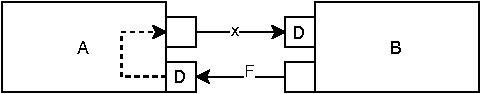
\includegraphics[width=0.5\textwidth]{images/simple_example.pdf}
    \end{figure}
\end{frame}

\begin{frame}{The precondition of Step(h):}
    \begin{itemize}
        \item All inputs should be set at the current SU-time t.
        \begin{itemize}
            \item Reactive inputs should be set with a value obtained at time $t+h$.
             \item Delayed inputs should be set with a value obtained at time $t$.
        \end{itemize}
        \item The SU should be capable of calculating its future state to time $t+h$. 
    \end{itemize}

    Affect on the global state:
    \begin{itemize}
        \item The SU advances to time $t+h$.
        \item All outputs get undefined and advance their time the new time.
    \end{itemize}
\end{frame}


\begin{frame}{The precondition of Get for port O:}
    \begin{itemize}
        \item All inputs that feed-through to O should be set at the same time as the SU.
    \end{itemize}
    Affect on the global state:
    \begin{itemize}
        \item The Output gets defined at the current time.
    \end{itemize}
\end{frame}

\begin{frame}{The precondition of Set for port I:}
    \begin{itemize}
        \item if Reactive:
        \begin{itemize}
            \item The output that connects to I is defined at a greater time than I.
        \end{itemize}
        \item if Delayed:
        \begin{itemize}
            \item The output that connects to I is defined at the same time as I.
        \end{itemize}
    \end{itemize}
    Affect on the global state:
    \begin{itemize}
        \item The Input gets defined at the time of the connected output.
    \end{itemize}
\end{frame}



\begin{frame}{The current tool-chain}
    The tool-chain (\url{https://github.com/INTO-CPS-Association/Scenario-Verifier}) for verifying and synthesizing master algorithms.
    \begin{figure}    
        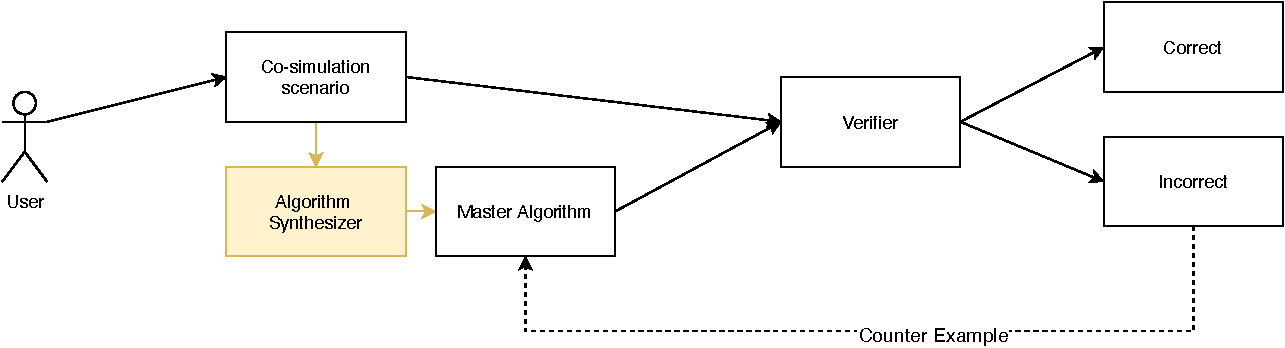
\includegraphics[width=0.95\textwidth]{images/usecase-synth.pdf}
    \end{figure}
    That will be integrated with Maestro2.
\end{frame}


\begin{frame}{Currrent Synthesizing strategy:}
    Graph-based approach, where:
    \begin{itemize}
        \item The SU-actions are the vertices.
        \item The constraints of the actions are the edges.
    \end{itemize}
    The topological order of the graph is the order of the actions. 
    \begin{columns}[T] % align columns
        \begin{column}{.48\textwidth}
            \begin{figure}    
                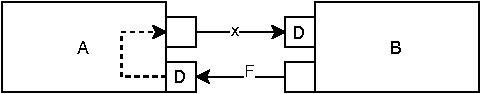
\includegraphics[width=0.9\textwidth]{images/simple_example.pdf}
            \end{figure}
            \vspace{-5mm}

            \begin{algorithm}[H]
                \caption{Step function:}
                \begin{algorithmic}[1]
                  \scriptsize
                  \State $\stateafter{A}{s+H} \gets \fdoStep{A}(\stateafter{A}{s}, H)$
                  \State $\stateafter{B}{s+H} \gets \fdoStep{B}(\stateafter{B}{s}, H)$
                  \State $F_v \gets \fget{B}(\stateafter{B}{s+H}, \outputvar{F})$
                  \State $\stateafter{A}{s+H} \gets \fset{A}(\stateafter{a}{s+H}, \inputvar{F}, F_v)$
                  \State $x_v \gets \fget{A}(\stateafter{A}{s+H}, \outputvar{x})$
                  \State $\stateafter{B}{s} \gets \fset{B}(\stateafter{B}{s+H}, \inputvar{x}, x_v)$
                \end{algorithmic}
              \end{algorithm}
    \end{column}%
    \hfill%
    \begin{column}{.48\textwidth}
        \begin{figure}
            \centering
            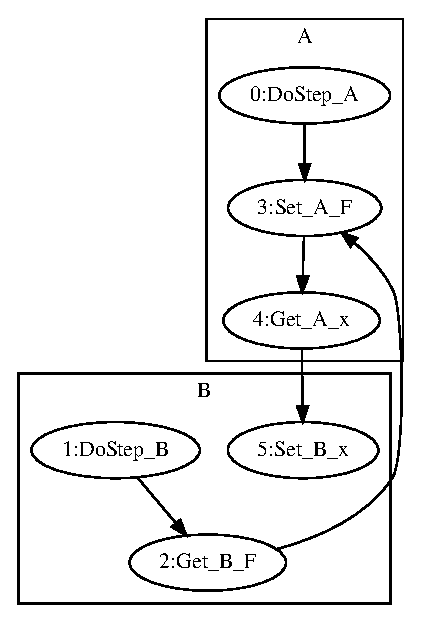
\includegraphics[width=0.6\textwidth]{images/simple_master_2_step.pdf}
        \end{figure}
    \end{column}%
    \end{columns}
\end{frame}

\begin{frame}{Simulation of complex scenario}
    \begin{columns}
        \begin{column}[]{0.5\textwidth}
            \begin{itemize}
                \item Should be simulated using a correct configuration (Step size + Fixed-points).
                \item An incorrect configuration breaks the preconditions.
                \item The simulation strategy is iteratively search for a correct (stable) configuration.
                \item The simulation is restarted after unsuccessful tries (using restore and save).
            \end{itemize}
        \end{column}
        \begin{column}[]{0.5\textwidth}
            \begin{algorithm}[H]
                \caption{Step negotiation}
            \label{alg:algorithm_step}
            \begin{algorithmic}[1]
              \scriptsize
                \While{$!\stepfound$} 
                \State $(\stateafter{D}{s+h_D},h_D) \gets \fdoStep{D}(\stateafter{D}{s}, h)$
                \State $g_v \gets \fget{D}(\stateafter{D}{s+h_D}, \outputvar{g})$       
                \State $\stateafter{C}{s} \gets \fset{C}(\stateafter{C}{s}, \inputvar{G}, G_v)$
                \State $(\stateafter{C}{s+h_C},h_C) \gets \fdoStep{C}(\stateafter{C}{s}, h_D)$
                \State $h \gets min(h_C, h_D)$
                \State $\stepfound \gets h == h_C \land h == h_D$
                \If{$!\stepfound$}
                    \State Restore SUs
                \EndIf
                \EndWhile
            \end{algorithmic} 
          \end{algorithm}
        \end{column}
    \end{columns}    
\end{frame}


\begin{frame}{Challenges in Synthesizing Algorithms}
    \begin{itemize}
        \item Complex Scenarios - having SCC in the graph.
        \begin{itemize}
            \item Solving Algebraic Loops (cycles in the graph)
            \item Performing Step Negotiation to ensure that SUs move in lockstep.
        \end{itemize}
    \end{itemize}
    These are solved using specialize heuristics to break the SCCs.
    \begin{columns}[T] 
        \begin{column}{.48\textwidth}
            \begin{figure}    
                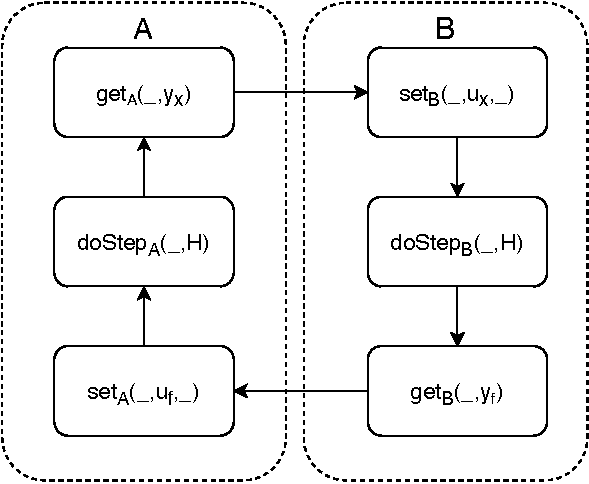
\includegraphics[width=0.9\textwidth]{images/reactive_step_graph.pdf}
            \end{figure}  
        \end{column}
    \hfill%
    \begin{column}{.48\textwidth}
        \begin{figure}    
            \centering
            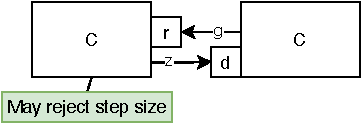
\includegraphics[width=0.9\textwidth]{images/step_scenario_org.pdf}
        \end{figure}
    \end{column}
    \end{columns}
\end{frame}

\begin{frame}{Synthesizing Complex Scenarios - Algebraic Loop}
    The SCC is broken using reduction scheme:
    \begin{columns}[T] 
        \begin{column}{.48\textwidth}
            \begin{figure}    
                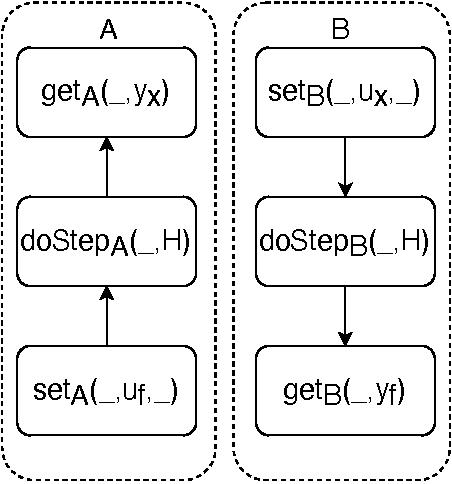
\includegraphics[width=0.8\textwidth]{images/jacobian_reduced_graph.pdf}
                \caption{Maximal reduction.}
            \end{figure}  
        \end{column}
    \hfill%
    \begin{column}{.48\textwidth}
        \begin{figure}    
            \centering
            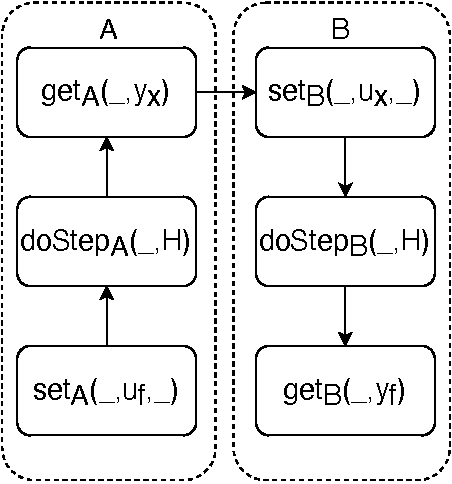
\includegraphics[width=0.8\textwidth]{images/gauss_reduced_graph.pdf}
            \caption{Minimal reduction.}
        \end{figure}
    \end{column}
    \end{columns}
\end{frame}


\begin{frame}{Synthesizing Complex Scenarios - Step negotiation}
    \begin{columns}[T] 
        \begin{column}{.48\textwidth}
            \begin{figure}    
                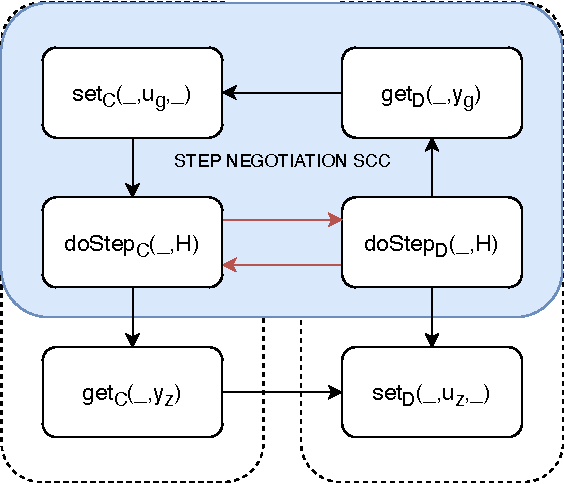
\includegraphics[width=0.8\textwidth]{images/step_scenario_graph.pdf}
                \caption{Step graph - the blue part shows the iterative search.}
            \end{figure}  
        \end{column}
    \hfill%
    \begin{column}{.48\textwidth}
        \begin{algorithm}[H]
            \caption{Step negotiation.}
        \begin{algorithmic}[1]
          \scriptsize
            \While{$!\stepfound$} 
            \State $(\stateafter{D}{s+h_D},h_D) \gets \fdoStep{D}(\stateafter{D}{s}, h)$
            \State $g_v \gets \fget{D}(\stateafter{D}{s+h_D}, \outputvar{g})$       
            \State $\stateafter{C}{s} \gets \fset{C}(\stateafter{C}{s}, \inputvar{G}, G_v)$
            \State $(\stateafter{C}{s+h_C},h_C) \gets \fdoStep{C}(\stateafter{C}{s}, h_D)$
            \State $h \gets min(h_C, h_D)$
            \State $\stepfound \gets h == h_C \land h == h_D$
            \If{$!\stepfound$}
                \State Restore SUs
            \EndIf
            \EndWhile
        \end{algorithmic} 
      \end{algorithm}
    \end{column}
    \end{columns}
\end{frame}

\begin{frame}{Verification of an OA}
    We want to ensure:
    \begin{itemize}
        \item All preconditions are satisfied
        \item The algorithm should follow the FMI-standard
    \end{itemize}
\end{frame}

\begin{frame}{Current Verification Strategy}
    The user specify a scenario and algorithm in DSL: 
    \begin{figure}    
        \centering
        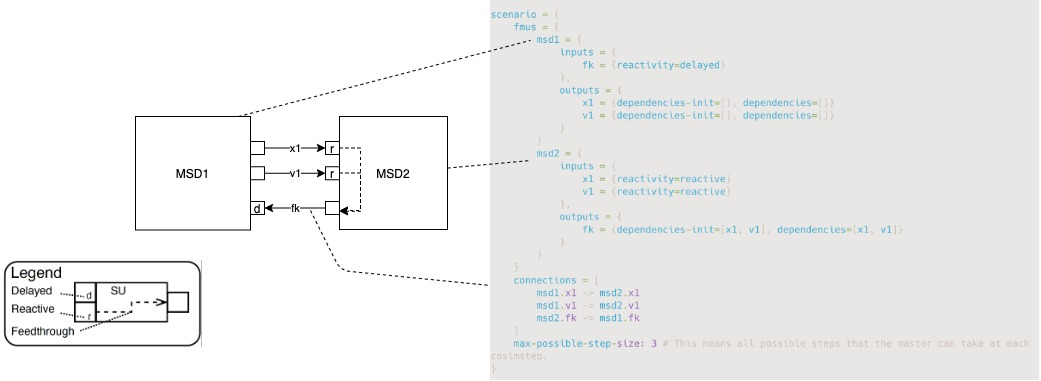
\includegraphics[width=0.9\textwidth]{images/scenario-generation.jpg}
    \end{figure}
    The tool instantiates a symbolic encoding of a co-simulation in UPPAAL-model to check that no preconditions are violated and that the algorithm follows the FMI-standard.
\end{frame}

\begin{frame}{UPPAAL model}
    \begin{itemize}
        \item Consist of 4 templates:
        \begin{itemize}
            \item An Orchestrator run the algorithm
            \item SUs that model the interface of an SU
            \item A template to verify Algebraic Loops
            \item A template to verify Step Negotiation
        \end{itemize}
    \end{itemize}
    \begin{figure}
        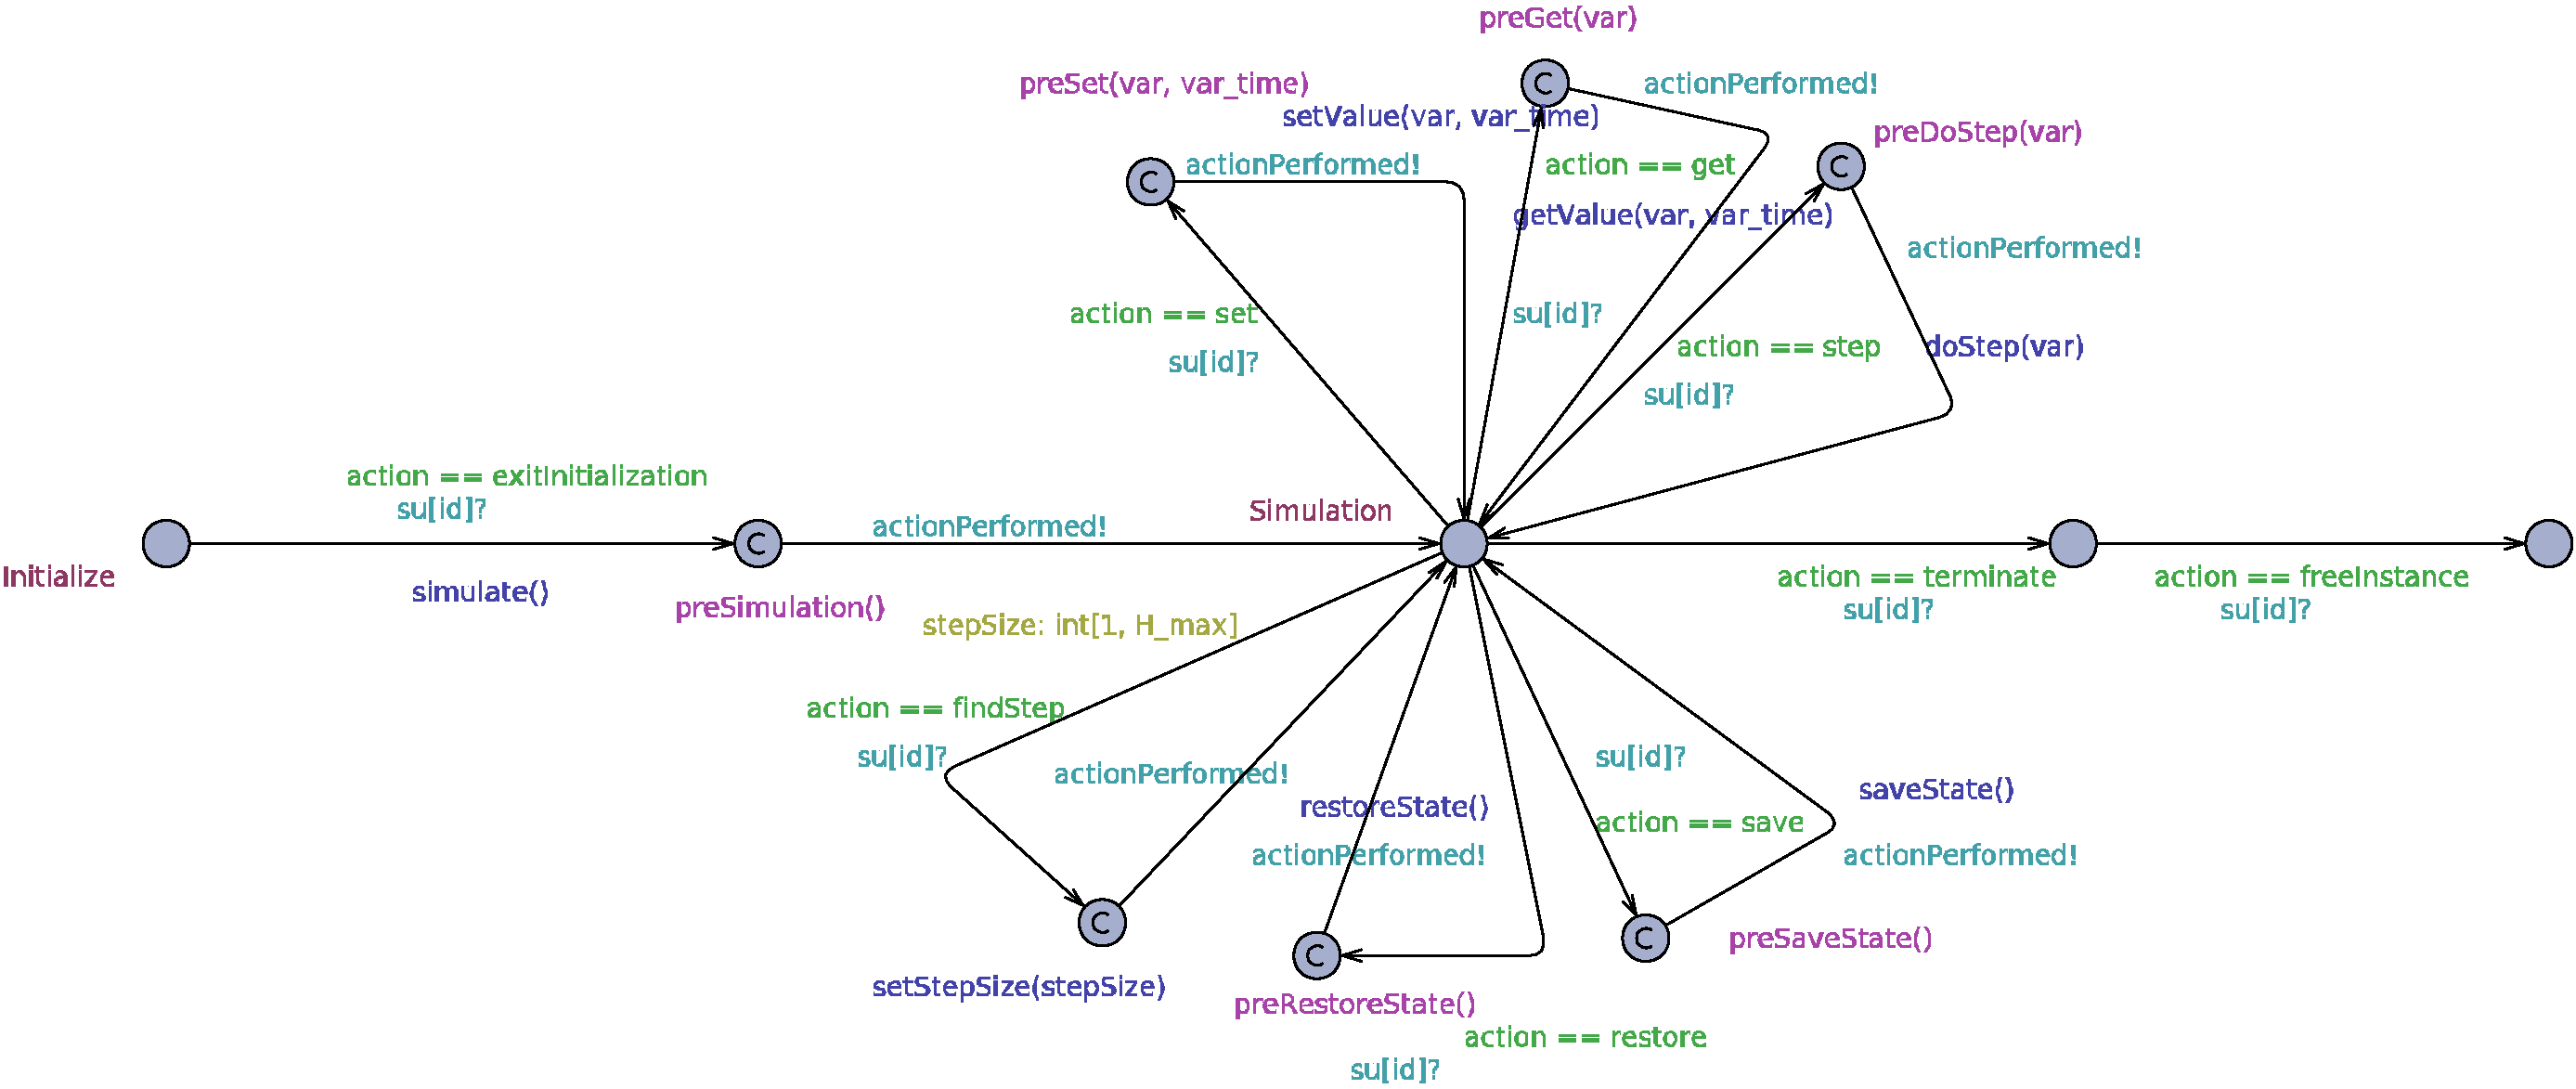
\includegraphics[width=0.9\textwidth]{images/SU_snippet.pdf}
        \caption{The SU template.}
    \end{figure}
\end{frame}


\section{The use of Maude}

\begin{frame}{Rewriting in Maude}
    \begin{enumerate}
        \item We could encode the preconditions of the actions as rewriting rules!
        \item Use Maude's model checker to rewrite the system and come up with a suitable algorithm.
        \item Combination of verification and synthesizing - correct by construction. 
        \item An elegant encoding of the problem.
    \end{enumerate}

    The challenge is the complex scenarios.
    \begin{itemize}
        \item The rewrite rules will from a graph with cycles.
        \item We need to capture the loops and use equivalence transformations to remove the cycles.
    \end{itemize}
\end{frame}

\begin{frame}{Maude encoding}
    Finding the right level of abstraction - should it be on the basis of ports or on SUs?
\begin{itemize}
    \item SU
    \begin{itemize}
        \item Id - Qid
        \item LocalTime - Nat - modulo 3
        \item Inputs - List of IId * Mode (set/notset) * Type (D/R) * feed-through (list of Outputs)
        \item Outputs - List of OId * Mode (defined/undefined)
        \item MayReject - Bool
    \end{itemize}
    \item Connections - List of Outputs * Inputs
    \item SimulationTime - Nat - modulo 3
\end{itemize}
\end{frame}

\begin{frame}{The next steps?}
    I have started a to encode scenarios in Maude.
    \begin{itemize}
        \item Simple scenario.
        \item 
    \end{itemize}   
\end{frame}


\end{document}